\documentclass[11pt,a4paper,oneside]{report}             % Single-side
%\documentclass[11pt,a4paper,twoside,openright]{report}  % Duplex

%\PassOptionsToPackage{chapternumber=Huordinal}{magyar.ldf}
\usepackage{t1enc}
\usepackage[latin2]{inputenc}
\usepackage{amsmath}
\usepackage{amssymb}
\usepackage{enumerate}
\usepackage[thmmarks]{ntheorem}
\usepackage{graphics}
\usepackage{epsfig}
\usepackage{listings}
\usepackage{color}
%\usepackage{fancyhdr}
\usepackage{lastpage}
\usepackage{anysize}
\usepackage[english]{babel}
\usepackage{sectsty}
\usepackage{setspace}  % Ettol a tablazatok, abrak, labjegyzetek maradnak 1-es sorkozzel!
\usepackage[hang]{caption}
\usepackage{hyperref}

%--------------------------------------------------------------------------------------
% Main variables
%--------------------------------------------------------------------------------------
\newcommand{\vikszerzo}{Kov\'acs \'Ad\'am}
\newcommand{\vikkonzulens}{Dr.~Recski G\'abor}
\newcommand{\vikcim}{Semantic parsing with graph transformations}
\newcommand{\viktanszek}{Department of Automation and Applied Informatics}
\newcommand{\vikdoktipus}{Master's Thesis}
\newcommand{\vikdepartmentr}{Kov\'acs \'Ad\'am}

%--------------------------------------------------------------------------------------
% Page layout setup
%--------------------------------------------------------------------------------------
% we need to redefine the pagestyle plain
% another possibility is to use the body of this command without \fancypagestyle
% and use \pagestyle{fancy} but in that case the special pages
% (like the ToC, the References, and the Chapter pages)remain in plane style

\pagestyle{plain}
%\setlength{\parindent}{0pt} % ?ttekinthet?bb, angol nyelv? dokumentumokban jellemz?
%\setlength{\parskip}{8pt plus 3pt minus 3pt} % ?ttekinthet?bb, angol nyelv? dokumentumokban jellemz?
\setlength{\parindent}{12pt} % magyar nyelv? dokumentumokban jellemz?
\setlength{\parskip}{0pt}    % magyar nyelv? dokumentumokban jellemz?

\marginsize{35mm}{25mm}{15mm}{15mm} % anysize package
\setcounter{secnumdepth}{0}
\sectionfont{\large\upshape\bfseries}
\setcounter{secnumdepth}{2}
\singlespacing
\frenchspacing

%--------------------------------------------------------------------------------------
%	Setup hyperref package
%--------------------------------------------------------------------------------------
\hypersetup{
    bookmarks=true,            % show bookmarks bar?
    unicode=false,             % non-Latin characters in Acrobat?s bookmarks
    pdftitle={\vikcim},        % title
    pdfauthor={\vikszerzo},    % author
    pdfsubject={\vikdoktipus}, % subject of the document
    pdfcreator={\vikszerzo},   % creator of the document
    pdfproducer={Producer},    % producer of the document
    pdfkeywords={keywords},    % list of keywords
    pdfnewwindow=true,         % links in new window
    colorlinks=true,           % false: boxed links; true: colored links
    linkcolor=black,           % color of internal links
    citecolor=black,           % color of links to bibliography
    filecolor=black,           % color of file links
    urlcolor=black             % color of external links
}

%--------------------------------------------------------------------------------------
% Set up listings
%--------------------------------------------------------------------------------------
\lstset{
	basicstyle=\scriptsize\ttfamily, % print whole listing small
	keywordstyle=\color{black}\bfseries\underbar, % underlined bold black keywords
	identifierstyle=, 					% nothing happens
	commentstyle=\color{white}, % white comments
	stringstyle=\scriptsize\sffamily, 			% typewriter type for strings
	showstringspaces=false,     % no special string spaces
	aboveskip=3pt,
	belowskip=3pt,
	columns=fixed,
	backgroundcolor=\color{lightgray},
} 		
\def\lstlistingname{lista}	

%--------------------------------------------------------------------------------------
%	Some new commands and declarations
%--------------------------------------------------------------------------------------
\newcommand{\code}[1]{{\upshape\ttfamily\scriptsize\indent #1}}

% define references
\newcommand{\figref}[1]{\ref{fig:#1}.}
\renewcommand{\eqref}[1]{(\ref{eq:#1})}
\newcommand{\listref}[1]{\ref{listing:#1}.}
\newcommand{\sectref}[1]{\ref{sect:#1}}
\newcommand{\tabref}[1]{\ref{tab:#1}.}

\DeclareMathOperator*{\argmax}{arg\,max}
%\DeclareMathOperator*[1]{\floor}{arg\,max}
\DeclareMathOperator{\sign}{sgn}
\DeclareMathOperator{\rot}{rot}
\definecolor{lightgray}{rgb}{0.95,0.95,0.95}

\author{\vikszerzo}
\title{\viktitle}
\includeonly{
	guideline,%
	project,%
	titlepage,%
	declaration,%
	abstract,%
	introduction,%
	chapter1,%
	chapter2,%
	chapter3,%
	acknowledgement,%
	appendices,%
}
%--------------------------------------------------------------------------------------
%	Setup captions
%--------------------------------------------------------------------------------------
\captionsetup[figure]{
%labelsep=none,
%font={footnotesize,it},
%justification=justified,
width=.75\textwidth,
aboveskip=10pt}

\renewcommand{\captionlabelfont}{\small\bf}
\renewcommand{\captionfont}{\footnotesize\it}

%--------------------------------------------------------------------------------------
% Table of contents and the main text
%--------------------------------------------------------------------------------------
\begin{document}
\singlespacing
\pagenumbering{arabic}
\onehalfspacing
%--------------------------------------------------------------------------------------
%	The title page
%--------------------------------------------------------------------------------------
\begin{titlepage}
\begin{center}

\includegraphics[width=60mm,keepaspectratio]{figures/BMElogo.png}\\
\vspace{0.3cm}
\textbf{Budapesti M�szaki �s Gazdas�gtudom�nyi Egyetem}\\
\textmd{Villamosm�rn�ki �s Informatikai Kar}\\
\textmd{\viktanszek}\\[5cm]

\vspace{0.4cm}
{\huge \bfseries \vikcim}\\[0.8cm]
\vspace{0.5cm}
\textsc{\Large \vikdoktipus}\\[4cm]

\begin{tabular}{cc}
 \makebox[7cm]{\emph{Author}} & \makebox[7cm]{\emph{Supervisor}} \\
 \makebox[7cm]{\vikszerzo} & \makebox[7cm]{\vikkonzulens}
\end{tabular}

\vfill
{\large \today}
\end{center}
\end{titlepage}



\tableofcontents\vfill
%--------------------------------------------------------------------------------------
% Nyilatkozat
%--------------------------------------------------------------------------------------
\begin{center}
\large
\textbf{HALLGAT�I NYILATKOZAT}\\
\end{center}

Alul�rott \emph{\vikszerzo}, szigorl� hallgat� kijelentem, hogy ezt a diplomatervet meg nem engedett seg�ts�g n�lk�l, saj�t magam k�sz�tettem, csak a megadott forr�sokat (szakirodalom, eszk�z�k stb.) haszn�ltam fel. Minden olyan r�szt, melyet sz� szerint, vagy azonos �rtelemben, de �tfogalmazva m�s forr�sb�l �tvettem, egy�rtelm�en, a forr�s megad�s�val megjel�ltem.

Hozz�j�rulok, hogy a jelen munk�m alapadatait (szerz�(k), c�m, angol �s magyar nyelv� tartalmi kivonat, k�sz�t�s �ve, konzulens(ek) neve) a BME VIK nyilv�nosan hozz�f�rhet� elektronikus form�ban, a munka teljes sz�veg�t pedig az egyetem bels� h�l�zat�n kereszt�l (vagy autentik�lt felhaszn�l�k sz�m�ra) k�zz�tegye. Kijelentem, hogy a beny�jtott munka �s annak elektronikus verzi�ja megegyezik. D�k�ni enged�llyel titkos�tott diplomatervek eset�n a dolgozat sz�vege csak 3 �v eltelte ut�n v�lik hozz�f�rhet�v�.

\begin{flushleft}
\vspace*{1cm}
Budapest, \today
\end{flushleft}

\begin{flushright}
 \vspace*{1cm}
 \makebox[7cm]{\rule{6cm}{.4pt}}\\
 \makebox[7cm]{\emph{\vikszerzo}}\\
 \makebox[7cm]{hallgat�}
\end{flushright}
\thispagestyle{empty}

\vfill
\clearpage
\thispagestyle{empty} % an empty page


%----------------------------------------------------------------------------
% Abstract in hungarian
%----------------------------------------------------------------------------
\chapter*{Kivonat}\addcontentsline{toc}{chapter}{Kivonat}
A term�szetes nyelvfeldolgoz�s a g�pi tanul�s egy olyan �ga, ami term�szetes nyelv sz�m�t�g�ppel val� feldolgoz�s�hoz 
elengedhetetlen eszk�z�ket ny�jt, �s a modern vil�gunkban egyre ink�bb elterjedt� v�lik a g�p �s az emberek k�z�tti
term�szetes nyelven t�rt�n� kommunik�ci�ra. Ennek megval�s�t�s�hoz van sz�ks�g�nk a sz�veg tartalmi elemz�s�re.

A szemantikai elemz�s (semantic parsing) c�lja, hogy nyers sz�veges adathoz automatikusan
k�sz�thess�nk szemantikai reprezent�ci�t, azaz modellezz�k a sz�veg jelent�s�t. Ha a nyelvi
jelent�st fogalmak ir�ny�tott gr�fjaival reprezent�ljuk, ezeket pedig a mondat szintaktikai
szerkezet�t reprezent�l� f�kb�l kell el��ll�tanunk, akkor a teljes feladat egyetlen komplex gr�ftranszform�ci�k�nt
defini�lhat�.

Egy-egy ilyen elemz� teljes�tm�nye k�zvetlen�l nem, csak konkr�t technol�gi�kon kereszt�l 
�rt�kelhet�, ilyen p�ld�ul a g�pi sz�veg�rt�s (Machine Comprehension) vagy a term�szetes nyelvi k�vetkeztet�s (Natural Language Inference)
, illetve tud�sb�zis popul�ci� (Knowledge Base Population). A m�ly szemantikai elemz�s elker�lhetetlen r�sze a lexik�lis k�vetkeztet�s (lexical inference),
melynek sor�n egy-egy sz� jelent�s�nek reprezent�ci�j�b�l kiindulva pr�b�ljuk b�v�teni az egy eg�sz fr�zis vagy mondat jelent�s�t reprezent�l� gr�fot.

A diplomaterv t�m�ja az el�bb eml�tett feladatok megold�sa a szemantika elemz� \texttt{4lang} \cite{Recski:2016d} rendszer seg�ts�g�vel, illetve ennek b�v�t�se
megfelel� inferenci�t megval�s�t� szab�lyokkal �s a gr�fok felett �rtelmezett metrik�kkal. A dolgozat mag�ba fogalja a 4lang rendszer lehet�s�geinek
REST API-t megval�s�t� mikroszolg�ltat�sokba val� csomagol�s�t is. 

A g�pi sz�veg�rt�s feladaton a kidolgozott rendszer�nk el�zetes eredm�nyei kis javul�st mutatnak a 2018-ban bemutatott state-of-the art rendszerhez \cite{Wang:2018} k�pest.
\vfill

%----------------------------------------------------------------------------
% Abstract in english
%----------------------------------------------------------------------------
\chapter*{Abstract}\addcontentsline{toc}{chapter}{Abstract}

Natural language processing (NLP) is a branch of machine learning that provides us tools for analyzing raw text automatically. 
In our modern world human-machine communication has become a widely required task. In order to meet it's requirements, it is inevitable to analyze
the text's meaning.

The main task of semantic parsing is to automatically build semantic representation from the input, so we can model the meaning
of raw texts. If we model meaning as directed graphs of concept and we can build them from syntax trees that represents the structure of 
sentences, then we can define the whole process as one complex graph transformation.

The performance of such analyzers cannot be measured directly, only through concrete tasks, such as Machine comprehension, 
Natural language inference, or Knowledge base population. Lexical inference has a very strong connection to deep semantic parsing, 
where we want to augment the graph that represents the meaning of a concept or a sentence by taking each word's graph that models its meaning. 

The main focus of this thesis is to give a strong baseline for the task mentioned above, and to enchahnt existing systems
with the help of the semantic parser \texttt{4lang} \cite{Recski:2016d}. We believe
the significance of these experiments lies in its
demonstration that inference based graph transformations are a powerful method for solving any semantic parsing related task.
The thesis includes the improving of the 4lang system with further inference based rules and various metrics related to semantic graphs. Furthermore it will demonstrate
the wrapping the 4lang software in Restful Wep Api microservices for easier usage.   

The biggest result of this paper is that our system's preliminary results suggest that our system achieves a .5
percentage point improvement on the Machine Comprehension task over the original state-of-the art system. 
\vfill


\chapter{Introduction}
\label{chap:Introdu}
In modern systems distributional models are dominant for a semantic parser. In my thesis I use graph based methods and 
apply it to various tasks, e.g. \textit{Knowledge base population}, \textit{Natural language inference} and \textit{2018 Semeval task on Machine Comprehension} (MC), which was a combined work of Kov\'acs \'Ad\'am and G\'emes Kinga.
I built a REST-API (available at \url{http://hlt.bme.hu/4lang}) 
around the \textbf{4lang}\cite{Recski:2016} (described in Chapter \ref{chap:semanticparsing}) 
to present a highly automated process constructing semantic models from raw input, and I introduced simple inference rules and metrics to enchance the graphs and calculate similarities between them.
Online demo of the service is available at \url{http://4lang.hlt.bme.hu}. 
In Chapter \ref{chap:comprehension} I introduce a strong baseline for the task, 
followed by an enhancement of a state-of-the-art system \cite{Wang:2018} (Chapter \ref{chap:yuanfudao}). 
In this chapter we discuss the history of the Natural Language Processing (NLP) applications, 
and briefly define the structure of this paper.
%----------------------------------------------------------------------------
\section{Natural Language Processing}
While computers can be easily programmed to understand structured data, such as tables and spreadsheets, it can be rather challenging for them
to understand human communication. Because there is a vast difference in the magnitude of the unstructured data compared to the structured ones, there is a high demand
for tools, that can deal with raw text. That's where NLP comes in. It contains high variety of tools, that we have to use, when we need to deal with natural input.

Every day, we come into contact with human communication, we say a lot of words to other people, and they try to interpret them even when the context of the saying 
isn't necessarily complete. The listeners can use their common knowledge to fill the needed information. We resolve ambiguities, misunderstanding, and can even understand words 
we have never heard before just from the context of the communication.
Even though these tasks are trivial for us, for a computer it can be really hard.

%--------------------------------------------------------------------------------------
% egyszer� multtol jelenig bevezeto
The interest in NLP research began in the 1950s, the early phase was mainly focused on MT (Machine Translation), because after the World War II, people
recognized the importance of the translation from one language to another, and hoped to do it automatically.
However MT is still very difficult nowadays, so these researches discovered the main challenges of the syntactic and semantic parsing early.
As time passed, researches embraced new areas of NLP as more advanced technology and knowledge became available. Now that we live in a world where
computers and smartphones are widely accessible, collecting data became incredibly easy, as a result, statistical NLP drew attention because these models thrive off big data, but one cannot ignore 
simple rule based methods which can also be very powerful, especially using them as a hybrid model with statistical methods.
%--------------------------------------------------------------------------------------
% r�vid nlp pipeline

Building NLP applications requires many levels of analysis.
The typical pipeline is structured as follows:
\begin{itemize}
	\item First we need to tokenize our input text, which means breaking up the text into meaningful elements, especially into words
	\item After we tokenized our text, we need to perform word analysis called \texttt{morphology}, which is concerned with the structure of words.
	\item Part of speech assigns words to syntax behavior in a sentence.
	\item The main task of syntactic parsing is to analyze the grammatical structure of a sentence. Given a set of words, a parser forms units (subjects, verbs, etc..) according to some grammatical formalism.
	There are two main types of syntactic parsers:
	\begin{itemize}
		\item \textit{Constituency parsers} produce trees, that represent the grammatical structure.
		\item \textit{Dependency parsers} are the more popular nowadays. They represent the structure of a sentence as a dependency tree, which instead of grammatical relations, tries to model the dependencies between words.
	\end{itemize}
	A parse of the example sentence: \textit{"John has finished the work"} can be seen in Figure \ref{fig:johnfinished}.
	
	\item At this point we have various ways to analyze a text, but without modeling its \texttt{meaning}. Semantics is the study of meaning, and semantic parsing is a task to find a representation and assign it to the text. This task will be the main topic of our work.
\end{itemize}

\begin{figure*}[h!]
	\centering
	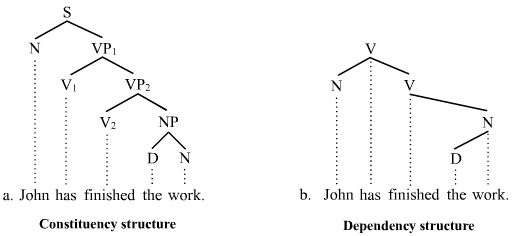
\includegraphics[width=0.7\textwidth]{figures/Johnhasfinishedthework}
	\caption{Parses of the sentence \textit{"John has finished the work"} \cite{parsers}}
	\label{fig:johnfinished}
\end{figure*}
%-------------------------------------------------------------
\section{Objectives}
The main focus of this study is computational semantics. My research includes building explicit representations of natural language semantics, because in today's state-of-the art systems for popular semantics tasks such as measuring semantic similarity or machine comprehension, they are rarely present. Virtually all systems
competing at popular challenges (e.g. \cite{Cer:2017,Collados:2017}) rely on word embeddings as the sole representation of word meaning. Recently \cite{Recski:2016c} has presented a method using graphical representations of natural language text that improved over the state-of-the art on the task of
measuring semantic similarity of pairs of English words. In this thesis
I use similar graphs as simple but powerful tools for measuring textual
entailment. My task includes defining new inference rules and methods for measuring graph similarities, and building an online available service for building graphs highly automatically, giving us a tool for building strong baseline methods. My work was based upon measuring our models through various semantic tasks such as Knowledge base population or the state-of-the art system on the 2018 Semeval Task \textit{Machine comprehension using commonsense knowledge}.

\section{Results}
We present a novel method for recognizing entailment using semantic
graphs and apply it to the tasks:
\begin{itemize}
    \item Knowledge base population task (KBP)
    \item 2017 RepEval task on Natural language inference (NLI)
    \item 2018 Semeval task on Machine
    Comprehension (MC).
\end{itemize}
First we present a highly automated process of building concept graphs from raw text building a microservice.
For the tasks I used the automatically built Concept graphs using the REST-API I defined based on the semantic parsing system \texttt{4lang} \cite{Recski:2016d}.
In the case of the KBP task I present a set of pilot experiments for augmenting a generic, open-domain 
knowledge base using a graph-based lexical ontology of English and simple
inference rules yielding millions of new facts with high
accuracy (over 90\% according to manual evaluation), the result was already presented in \cite{Kovacs:2018}.
For the NLI and MC task a strong baseline is presented using only concept graphs achieving accuracy scores of $67.5\%$ and $68.3\%$ respectively.
Followed by an enhancement of a state-of-the art system
\cite{Wang:2018}, where we proceeded to use the metric underlying our baseline as an additional feature. Preliminary results suggest that these features achieve a .5 percentage point improvement over the original system. This result was the output of the combined work with G\'emes Kinga presented in \cite{Kovacs:2018b}.

\section{References}
The code of the system is available on Github\footnote{\url{https://github.com/adaamko/4lang}}. The code was implemented by the author of this paper based upon the \textbf{4lang} system.

\section{Structure}
The structure of the paper is the following:
\begin{itemize}
	\item \textbf{Chapter \ref{chap:Introdu}} describes the short history and motivation of the NLP applications, it also gives a short summary about the objectives of the thesis, and the results.
	\item \textbf{Chapter \ref{chap:semanticparsing}} gives a short introduction into the field of semantic parsing, and semantic models in general. It briefly explains the semantic parsing system \textbf{4lang}, and my process of automating the building of concept graphs, and the newly defined inference methods
	\item \textbf{Chapter \ref{chap:comprehension}} describes the baseline approach to the Machine Comprehension task, which achieved an accuracy score of $68.3\%$.
	\item \textbf{Chapter \ref{chap:deep}} gives an introduction into deep learning, focusing on the NLP tasks.
	\item \textbf{Chapter \ref{chap:yuanfudao}} presents our experiments with the state-of-the art system \textbf{Yuanfudao}. Our preliminary results show a .5 percent improvement over the original system.
	\item \textbf{Chapter \ref{chap:future}} summarizes our contributions and describes our ongoing/future work. It briefly discusses our plans for the follow-up, that was beyond the scope of this work.
\end{itemize}

\section{Division of labour}
This project was a product of the combined work of Kov\'acs \'Ad\'am and G\'emes Kinga. Kov\'acs \'Ad\'am was responsible for building the service to automate the process of building concept graphs (online demo available at \url{http://4lang.hlt.bme.hu}), and was mostly working on the baseline methods and defining new inference rules and metrics for the given tasks. G\'emes Kinga's main work involved applying the baseline to the state-of-the-art system Yuanfudao \cite{Wang:2018}\footnote{\url{https://github.com/GKingA/commonsense-rc}} and experiments with IRTGs briefly described in Chapter \ref{chap:future}\footnote{\url{https://github.com/GKingA/irtg}}.
%----------------------------------------------------------------------------
\chapter*{Acknowledgement}\addcontentsline{toc}{chapter}{Acknowledgement}
%----------------------------------------------------------------------------
First of all, 
I would like to express my deep gratitude to Dr. Recski G�bor for his guidance not just through this thesis, but through my whole master studies. I would like to thank him for introducing me to this interesting and amazing research field. He was always flexible and available for all my questions. I thank him for his valuable advices just about any topic imaginable.  

I am also thankful to Dr. Kornai Andr�s for his constant support
and help with my work. I thank him for his energy to discuss any of problems I have.

I also would like to thank to my colleague G�mes Kinga for her excellent work. 

Finally, a special thanks to my girlfriend for her constant love and support. I thank her for her supporting me even through difficult situations. Without her, I would not have been able to write this thesis.

%\listoffigures\addcontentsline{toc}{chapter}{?br?k jegyz?ke}
%\listoftables\addcontentsline{toc}{chapter}{T?bl?zatok jegyz?ke}

\bibliography{mybib}
\addcontentsline{toc}{chapter}{Bibliography}
\bibliographystyle{plain}

\label{page:last}
\end{document}
